\documentclass[a4paper,12pt]{article} %размер бумаги устанавливаем А4, шрифт 12пунктов
% \usepackage[T2A]{fontenc}
\usepackage[utf8]{inputenc}%кодировка
\usepackage[english,russian]{babel}%используем русский и английский языки с переносами
% \usepackage{amssymb,amsfonts,amsmath,cite,enumerate,float,indentfirst} %пакеты расширений
\usepackage[pdftex]{graphicx} %вставка графики
\graphicspath{{images/}}%путь к рисункам
% \usepackage{minted}
\usepackage{listings}
\usepackage{subcaption}

\usepackage{algorithmicx}
\usepackage{algpseudocode}
% \floatname{algorithm}{Procedure}

% \usepackage{algorithm2e}
%  % Перевод плагина
\SetKwInput{KwData}{Исходные параметры}
\SetKwInput{KwResult}{Результат}
\SetKwInput{KwIn}{Входные данные}
\SetKwInput{KwOut}{Выходные данные}
\SetKwIF{If}{ElseIf}{Else}{Если}{тогда}{иначе\ если}{иначе}{конец\ условия}
\SetKwFor{While}{До\ тех\ пор,\ пока}{выполнять}{конец\ цикла}
\SetKw{KwTo}{от}
\SetKw{KwRet}{возвратить}
\SetKw{Return}{Возвратить}
\SetKwBlock{Begin}{Начало\ блока}{конец\ блока}
\SetKwSwitch{Switch}{Case}{Other}{Проверить\ значение}{и\ выполнить}{вариант}{в\ противном\ случае}{конец\ варианта}{конец\ проверки\ значений}
\SetKwFor{For}{Цикл}{выполнять}{Конец\ цикла}
\SetKwFor{ForEach}{Для\ каждого}{выполнять}{Конец\ цикла}
\SetKwRepeat{Repeat}{Повторять}{До\ тех\ пор,\ пока}
\SetAlgorithmName{Алгоритм}{алгоритм}{Список алгоритмов}


% \makeatletter
% \renewcommand{\@biblabel}[1]{#1.} % Заменяем библиографию с квадратных скобок на точку:
% \makeatother

\usepackage{geometry} % Меняем поля страницы
\geometry{left=2.5cm}% левое поле
\geometry{right=1.5cm}% правое поле
\geometry{top=2cm}% верхнее поле
\geometry{bottom=2cm}% нижнее поле

% \usepackage{hyperref}
% \hypersetup{%
%     pdfborder = {0 0 0}
% }
\usepackage[hidelinks]{hyperref}

% \usepackage{wrapfig}

% \renewcommand{\theenumi}{\arabic{enumi}}% Меняем везде перечисления на цифра.цифра
% \renewcommand{\labelenumi}{\arabic{enumi}}% Меняем везде перечисления на цифра.цифра
% \renewcommand{\theenumii}{.\arabic{enumii}}% Меняем везде перечисления на цифра.цифра
% \renewcommand{\labelenumii}{\arabic{enumi}.\arabic{enumii}.}% Меняем везде перечисления на цифра.цифра
% \renewcommand{\theenumiii}{.\arabic{enumiii}}% Меняем везде перечисления на цифра.цифра
% \renewcommand{\labelenumiii}{\arabic{enumi}.\arabic{enumii}.\arabic{enumiii}.}% Меняем везде перечисления на цифра.цифра

% \newcommand{\imgh}[3]{\begin{figure}[h]\center{\includegraphics[width=#1]{#2}}\caption{#3}\label{ris:#2}\end{figure}}

\lstdefinelanguage{llang}{
	keywords={skip, do, while, read, write, if, then, else},
	sensitive=true,
	%%basicstyle=\small,
	commentstyle=\scriptsize\rmfamily,
	keywordstyle=\ttfamily\underbar,
	identifierstyle=\ttfamily,
	basewidth={0.5em,0.5em},
	columns=fixed,
	fontadjust=true,
	literate={->}{{$\to$}}1
}

\lstset{
	language=llang
}

\begin{document}
\begin{titlepage}
\newpage

\begin{center}
	\textbf{
		Санкт-Петербургский Государственный Университет \\
		Математико-механический факультет \\
	}
	Кафедра системного программирования
\end{center}

\vspace{15em}

\begin{center}
\Large Форматирование текста программ на основе комбинаторов, сопоставления с образцом и синтаксических шаблонов \\ 
\end{center}

\vspace{2em}

\begin{center}
Курсовая работа студента 445 группы \\
Подкопаева Антона Викторовича

% \textsc{\textbf{Название темы работы \linebreak длинное очень, набранное в \LaTeX{}}}
\end{center}

\vspace{10em}

Научный руководитель:\\
доцент кафедры системного программирования \dotfill
Д. Ю. Булычев

% \newbox{\lbox}
% \savebox{\lbox}{\hbox{Пупкин Иван Иванович}}
% \newlength{\maxl}
% \setlength{\maxl}{\wd\lbox}
% \hfill\parbox{11cm}{
% \hspace*{5cm}\hspace*{-5cm}Студент:\hfill\hbox to\maxl{Тест Пользователь\hfill}\\
% \hspace*{5cm}\hspace*{-5cm}Преподаватель:\hfill\hbox to\maxl{Пупкин Иван Иванович}\\
% \\
% \hspace*{5cm}\hspace*{-5cm}Группа:\hfill\hbox to\maxl{NNN}\\
% }


\vspace{\fill}

\begin{center}
Санкт-Петербург \\2013
\end{center}

\end{titlepage}

\newpage
\tableofcontents % это оглавление, которое генерируется автоматически
\newpage
\section*{Введение}
\addcontentsline{toc}{section}{Введение}

% На данный момент в программных системах самым распространенным представлением информации, которая создается пользователем или демонстрируется ему, является текстовое представление. Оно удобно по многим причинам, но у него есть существенный недостаток - часто без дополнительного стилизирования текстовая информация слишком тяжело воспринимается. При отображении данных для пользователя необходимо явственным образом сохранять изначальную структуру информации. В большинстве случаев такое стилизирование сводится к форматированию текста, то есть добавлению или удалению не несущих информацию символов, другому преобразованию текста без изменения его семантики. Данное преобразование называется \textbf{pretty printing}.

С появлением первых языков программирования особую важность приобрели языковые процессоры. \textbf{Языковой процессор} (\textbf{ЯП}) --- это программное средство, принимающее на вход программу в виде текста на некотором языке (программирования, разметки и т. д.) и решающее определенную задачу над этой программой. К языковым процессорам можно отнести: компиляторы, суперкомпиляторы, интерпретаторы, средства статического анализа кода, декомпиляторы, средства рефакторинга, средства реинжиниринга, интегрированные среды разработки (IDE) и др.

Первым этапом работы ЯП является \textbf{синтаксический анализ}, то есть сопоставление входного текста (линейной последовательности лексем) с формальной грамматикой языка. В результате работы синтаксического анализатора ЯП получает древовидное представление программы, над которым потом происходит основная работа.

Достаточно часто возникает задача показать пользователю промежуточный или конечный результат обработки кода.
Следовательно, необходимо вернуться к текстовому представлению программы, то есть провести процедуру, обратную синтаксическому анализу. Такая задача называется \textbf{pretty printing}, а соответствующий инструмент --- \textbf{pretty printer}. Далее этот инструмент мы будем называть \textbf{принтером}.

Одной из проблем, возникающей при разработке принтера, является то, что критерии качества его работы трудно формализуемы.
Очевидно, что одного соответствия с точки зрения синтаксиса и семантики полученного кода и древовидного представления недостаточно. Рассмотрим программы на рисунках~\ref{fig:wikiExUnfor} и \ref{fig:wikiExBSD}.

\begin{figure}[h!]
	\centering
	% \inputminted{c}{codes/wikiExUnfor.c}
	\lstinputlisting[language=C]{codes/wikiExUnfor.c}
	\caption{Неформатированный код}
	\label{fig:wikiExUnfor}
\end{figure}

\begin{figure}[h!]
	\centering
	% \inputminted{c}{codes/wikiExBSD.c}
	\lstinputlisting[language=C]{codes/wikiExBSD.c}
	\caption{Форматированный код}
	\label{fig:wikiExBSD}
\end{figure}

Они эквиваленты синтаксически и семантически с точки зрения компилятора C, но для пользователя вариант с рисунка~\ref{fig:wikiExBSD} предпочтительней, так как он проще для восприятия. Как мы видим, при отображении данных необходимо явным для пользователя образом сохранять иерархическую структуру информации. В большинстве случаев решение этой задачи сводится к добавлению или удалению символов, не несущих информации для синтаксического анализа, или другому преобразованию текста без изменения его семантики.

Кроме того определенную сложность в описание и исполнение конкретного принтера вносит тот факт, что в большинстве случаев нельзя однозначным образом сопоставить синтаксическую конструкцию с единственным представлением. Необходима вариативность в зависимости от дополнительных условий, наложенных на результат его работы.

Рассмотрим небольшой пример. Пользователь задает условие вида: “последовательные операторы пишутся на одной строке, если помещаются в N символов, а иначе --- на разных строках”.

\begin{figure}[h!]
	\centering
	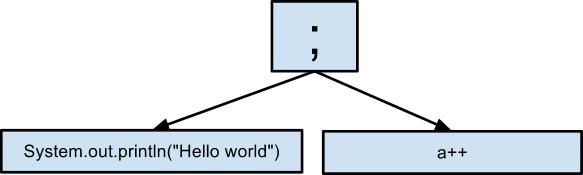
\includegraphics[width=0.8\textwidth]{seqTree}
	\caption{Последовательные операторы}
	\label{fig:seqImage}
\end{figure}

На рисунке~\ref{fig:seqImage} изображено синтаксическое дерево последовательности двух операторов. Такое дерево, согласно заданному правилу, может быть напечатано одним из двух вариантов (рисунки ~\ref{fig:seqCode1}, ~\ref{fig:seqCode2}).

\begin{figure}[h!]
	\centering
	% \inputminted{c}{codes/seqCode1.java}
	\lstinputlisting[language=Java]{codes/seqCode1.java}
	\caption{Последовательные операторы в строчку}
	\label{fig:seqCode1}
\end{figure}

\begin{figure}[h!]
	\centering
	% \inputminted{c}{codes/seqCode2.java}
	\lstinputlisting[language=Java]{codes/seqCode2.java}
	\caption{Последовательные операторы в несколько строк}
	\label{fig:seqCode2}
\end{figure}

Выбор происходит в зависимости от ширины вывода. Так, при ширине равной 35 символов (длина строки <<System.out.println(“Hello world”); >>), должен выбираться вариант, изображенный на рисунке~\ref{fig:seqCode2}, так как код на рисунке~\ref{fig:seqCode1} имеет ширину более 35 символов.
Могут быть заданы и более сложные условия.

Рассмотрим другой пример. Пусть нам нужно текстовое представление синтаксического дерева конструкции <<\lstinline{if}>>, и заданы шаблонами c рисунков~\ref{fig:ifTemplate2} и \ref{fig:ifTemplate1}, причем вариант, изображенный на рисунке~\ref{fig:ifTemplate2} выбирается в случае, если условие и ветки могут быть напечатаны в одну строчку.

\begin{figure}[h!]
	\begin{subfigure}[b]{0.45\textwidth}
		% \inputminted{haskell}{codes/ifTemplate2.hs}
		\lstinputlisting[language=Haskell]{codes/ifTemplate2.hs}
		\caption{}
		\label{fig:ifTemplate2}
	\end{subfigure}
	\hspace{1cm}
	\begin{subfigure}[b]{0.45\textwidth}
		% \inputminted{haskell}{codes/ifTemplate1.hs}
		\lstinputlisting[language=Haskell]{codes/ifTemplate1.hs}
		\caption{}
		\label{fig:ifTemplate1}
	\end{subfigure}
	\caption{Представления для конструкции <<\lstinline{if}>>}
\end{figure}


Тогда для деревьев, представленных на рисунках \ref{fig:ifImage1} и \ref{fig:ifImage2}, будут напечатаны коды с рисунков \ref{fig:ifCode1} и \ref{fig:ifCode2} соответственно.

\begin{figure}[h!]
	\begin{subfigure}[b]{0.60\linewidth}
		\centering
		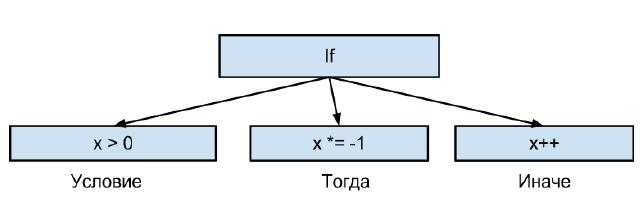
\includegraphics[width=\textwidth]{if1}
		\caption{}
		\label{fig:ifImage1}
	\end{subfigure}
	\hspace{0.5cm}
	\begin{subfigure}[b]{0.30\linewidth}
		\centering
		% \inputminted{haskell}{codes/ifCode1.hs}
		\lstinputlisting[language=Haskell]{codes/ifCode1.hs}
		\caption{}
		\label{fig:ifCode1}
	\end{subfigure}

	\caption{Использование представления с рис.~\ref{fig:ifTemplate2}}
\end{figure}

\begin{figure}[h!]
	\begin{subfigure}[b]{0.60\linewidth}
		\centering
		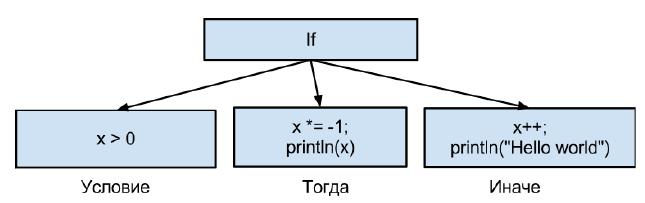
\includegraphics[width=\textwidth]{if2}
		\caption{}
		\label{fig:ifImage2}
	\end{subfigure}
	\hspace{0.5cm}
	\begin{subfigure}[b]{0.30\linewidth}
		\centering
		% \inputminted{haskell}{codes/ifCode2.hs}
		\lstinputlisting[language=Haskell]{codes/ifCode2.hs}
		\caption{}
		\label{fig:ifCode2}
	\end{subfigure}

	\caption{Использование представления с рис.~\ref{fig:ifTemplate1}}
\end{figure}

% Постановка задачи
То, что не существует четких критериев красоты кода, а также отсутствие библиотек, предоставляющих возможность описать принтер в виде, подобном
рассмотренному примеру с конструкцией <<\lstinline{if}>>, то есть с помощью шаблонов, часто приводит к тому, что принтеры становятся крайне сложными и наполненными эвристиками.

Задачей данной работы было изучение существующих подходов к построению принтеров в рамках функциональных языков программирования и разработка способа определения принтеров с помощью синтаксических шаблонов.
\newpage
\section{Обзор существующих библиотек}

В рамках исследования был проведен анализ существующих pretty printer библиотек на основе комбинаторов.
% возможно, рассказать о комбинаторах

\subsection{Библиотека Джона Хьюза}

Библиотека Джона Хьюза, описанная в \cite{hughes}, явялется первой комбинаторной pretty printing библиотекой. Она основана на алгоритме, предложенном Дереком Оппеном в \cite{oppen}, по сути является его реализацией в функциональном стиле на Haskell. Также библиотека Джона Хьюза, расширенная Саймоном Пейтоном Джонсом \cite{peytonJones}, является стандартной pretty print библиотекой для Haskell.

% рассказать об оптимальном

В данной библиотеке ключевым типом является \textbf{Doc}. Основные комбинаторы для составления документа:
\inputminted{haskell}{codes/hughesBasicOperators.hs}

Так с помощью функции \textbf{text} по строке получается документ, оператор \textbf{(<>)} соединяет два документа горизонтально (см. рисунок~\ref{fig:hughesHorComp}), а оператор \textbf{(\$\$)} соединяет документы вертикально (см. рисунок~\ref{fig:hughesVertComp}).

\begin{figure}[h!]
	\begin{minipage}[b]{0.45\linewidth}
		\centering
		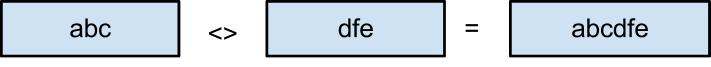
\includegraphics[width=\textwidth]{hughesHorComp}
		\caption{}
		\label{fig:hughesHorComp}
	\end{minipage}
	\hspace{0.5cm}
	\begin{minipage}[b]{0.45\linewidth}
		\centering
		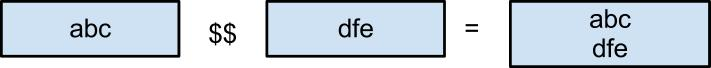
\includegraphics[width=\textwidth]{hughesVertComp}
		\caption{}
		\label{fig:hughesVertComp}
	\end{minipage}
\end{figure}

Элемент типа \textbf{Doc} может быть переведен в строку с помощью функции \textbf{pretty}.
\inputminted{haskell}{codes/hughesPretty.hs}
Кроме самого документа, функция \textbf{pretty} также принимает два числа: максимальную длину и максимальную наполненность строки. Здесь максимальная наполненность строки значит длину текста без выдущих пробельных символов.


\newpage
\section{Реализация принтера, основанного на шаблонах}

Основной целью данной работы была разработка прототипа принтера, который бы использовал для печати шаблоны.

\subsection{Описание общего подхода}

Работа принтера разбивается на два этапа: подготовка шаблонов и непосредственно печать синтаксического дерева.

На подготовительном этапе из файла с шаблонами языковых конструкций строится набор образцов. \textit{Образцом} назовем пару из текста шаблона и обобщенного синтаксического дерева шаблона. Дерево шаблона --- обобщенное, так как на месте некоторых узлов стоят специальные метки, которые хранят информацию об ограничениях на текстовое представление соответствующих узлов.

Во время основной фазы работы принтера дерево, которое необходимо непачатать, сравнивается с деревьями из образцов. В случае согласованности образца и дерева для печати используется текст образца, в который на места меток вставляются представления соответствующих поддеревьев.

% Благодаря шаблонам, необходимый результат получается просто и наглядно.

\subsection{Шаблон}

Внутри шаблона используется специальный язык разметки. Символы “\lstinline{@-}” на позиции поддерева синтаксической конструкции означают, что для применения данного шаблона поддерево должно быть напечатано в одну строку. Семантика символов “\lstinline{@* N @*}” совпадает с семантикой “\lstinline{@-}” с точностью до того, что напечатанное поддерево должно занимать строку длины не более N. Символы “\lstinline{@| @|}” означают, что соответствующее поддерево может быть напечатано и на нескольких строках. Для выделения отдельных шаблонов используются строки “\lstinline{t_start}”, “\lstinline{t_end}”.

Рассмотрим пример шаблонов для конструкции “\lstinline{write}” языка L (см. рис. \ref{fig:writeTmplt1} и \ref{fig:writeTmplt2}).
Эти шаблоны задают именно такое представление \lstinline{write}”, которого мы добивались в обзоре принтер-библиотек.

\begin{figure}[h!]
	\null\hfill
	\subfloat[]{
		\lstinputlisting{codes/writeTmplt1.l}
		\label{fig:writeTmplt1}	
	}
	\hfill
	\subfloat[]{
		\lstinputlisting{codes/writeTmplt2.l}
		\label{fig:writeTmplt2}
	}
	\hfill
	\null

	% \begin{subfigure}[h]{0.45\textwidth}
	% 	\lstinputlisting{codes/writeTmplt1.l}
	% 	\caption{}
	% 	\label{fig:writeTmplt1}
	% \end{subfigure}
	% \begin{subfigure}[h]{0.45\textwidth}
	% 	\lstinputlisting{codes/writeTmplt2.l}
	% 	\caption{}
	% 	\label{fig:writeTmplt2}
	% \end{subfigure}
	\caption{Шаблоны для конструкции “\lstinline{write}”}
\end{figure}

Рассмотрим шаблоны для конструкции “\lstinline{if-then-else}” (см. рис. \ref{fig:flatGoodIfTmplt} и \ref{fig:multBadIfTmplt}).
С помощью них можно напечатать дерево, изображенное на рисунке~\ref{fig:nestedIf} (см. рис. \ref{fig:nestedIfCode}).

\begin{figure}[h!]
	\subfloat[Однострочный вариант]{
		\lstinputlisting{codes/flatGoodIfTmplt.l}
		\label{fig:flatGoodIfTmplt}
	}
	\hfill
	\subfloat[Многострочный вариант]{
		\lstinputlisting{codes/multBadIfTmplt.l}
		\label{fig:multBadIfTmplt}
	}
	
	% \begin{subfigure}[h]{0.45\textwidth}
	% 	\lstinputlisting{codes/flatGoodIfTmplt.l}
	% 	\caption{Однострочный вариант}
	% 	\label{fig:flatGoodIfTmplt}
	% \end{subfigure}
	
	% \begin{subfigure}[h]{0.45\textwidth}
	% 	\lstinputlisting{codes/multBadIfTmplt.l}
	% 	\caption{Многострочный вариант}
	% 	\label{fig:multBadIfTmplt}
	% \end{subfigure}
	\caption{Шаблоны для конструкции “\lstinline{if-then-else}”}
	\label{fig:ifTmplt}
\end{figure}

\begin{figure}[h!]
	\centering
	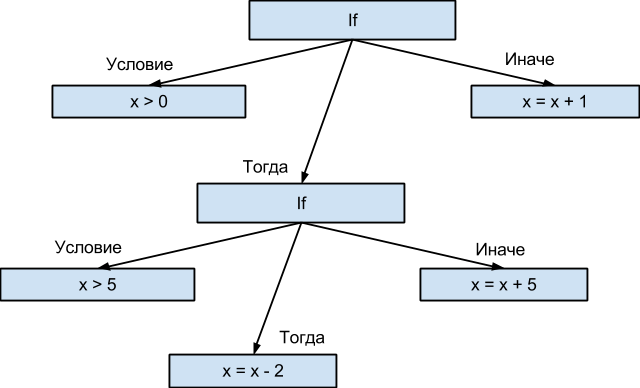
\includegraphics[width=0.6\textwidth]{nestedIf}
	\caption{Пример дерева “\lstinline{if-then-else}”}
	\label{fig:nestedIf}
\end{figure}

\begin{figure}[h!]
	\centering
	\lstinputlisting{codes/nestedIf.l}
	\caption{Представление с помощью шаблонов с рис. \ref{fig:ifTmplt}}
	\label{fig:nestedIfCode}
\end{figure}

Одним из неочевидных свойств шаблонов является то, что с их помощью можно выражать не только базовые конструкции языка.
Например, можно завести отдельный шаблон для случая, когда обе ветки конструкции “\lstinline{if-then-else}” представляют собой операторы “\lstinline{write}” (см. рис. \ref{fig:writeNestedInIf}). Если добавить такой шаблон, то пример дерева с рисунка~\ref{fig:nestedIf} получит новое представление (см. рис. \ref{fig:nestedIfNew}).

\begin{figure}[h!]
	\lstinputlisting{codes/writeNestedInIf.t}
	\caption{Пример задания шаблона для сложной конструкции}
	\label{fig:writeNestedInIf}
\end{figure}

\begin{figure}[h!]
	\lstinputlisting{codes/nestedIfNew.l}
	\caption{Представление дерева с рис. \ref{fig:nestedIf} с использованием шаблона с рис. \ref{fig:writeNestedInIf}}
	\label{fig:nestedIfNew}
\end{figure}

\subsection{Построение образцов}

Для работы принтера неообходимо иметь возможность сравнивать синтаксическое представление шаблонов с деревом, которое печатается. Поэтому необходим синтаксический анализатор, который может разбирать шаблонные конструкции в рамках целевого языка. Удобным способом разработать данный анализатор является использование расширяемого синтаксического анализатора целевого языка. В результате работы расширенного анализатора получается набор образцов. В узлах синтаксического дерева, соответствующих меткам шаблонов, хранится информация о положении метки внутри текста образца, чтобы на этапе печати документа знать, куда вставлять представления поддеревьев.

\newpage

\subsection{Печать дерева с использованием набора образцов}

На этапе, когда уже имеются необходимые образцы, происходит их сопоставление с синтаксическим деревом, переданным на печать.
Псевдокод алгоритма приведен ниже (см. рис. \ref{fig:comparePseudoCode}).

\begin{figure}[h!]
	\begin{algorithmic}
		\State{H --- ассоциативный массив, связывает деревья с их текстовым представлением}
		\State{M --- набор образцов для языковых конструкций}

		\State{ }
		\State{Комментарий: По дереву строит его текстовое представление}
		\Function{print}{$tree$}
			\If{$tree \in H$}
				\State\Return{$H[tree]$}
			\Else
				\State{Вызов print для поддеревьев $tree$}
				\State\Return{\Call{templateIter}{$tree$}}
			\EndIf
		\EndFunction

		\State{ }
		\State{Комментарий: Перебирает все образцы и пытается их применить к дереву}
		\Function{templateIter}{$tree$}
			\ForAll{$(templateTree, text) \in M$}
				\State{Комментарий: В случае исключения, переходит к новому элементу $M$}
				\State{$list$ := \Call{templateCompare}{$tree, templateTree$}}
				\State{$H[tree]$ := построенное представление для $tree$ по $list$ и $text$}
				\State\Return{$H[tree]$}
			\EndFor
		\EndFunction

		\State{ }
		\State{Комментарий: Возвращает список координат метки в тексте шаблона и соответствующее текстовое представление поддерева}
		\Function{templateCompare}{$tree, templateTree$}
			\If{$tree$ и $templateTree$ одного типа}
				\State{Вызвать $templateCompare$ для соответствующих поддеревьев}
				\State\Return{соединенный список результатов вызова для поддеревьев}
			\EndIf

			\If{$templateTree$ является меткой}
				\If{$H[tree]$ соответствует ограничениям метки}
					\State\Return{$[($координаты метки$, H[tree])]$}
				\Else
					\State{создать исключение}
				\EndIf
			\EndIf

			\State{Создать исключение, т.к. переданные деревья разной структуры}
		\EndFunction
		
	\end{algorithmic}
	\caption{Псевдокод сопоставления дерева с набором образцов}
	\label{fig:comparePseudoCode}
\end{figure}

Из псевдокода видно, что в случае, если для какого-нибудь поддерева не найдется соответствующий образец, то дерево невозможно будет напечатать. То есть множество образцов должно быть достаточным. Это естественное ограничение.

% Попробуем оценить время работы алгоритма. Пусть $|M|$ --- количество образцов, $height(T)$ --- высота дерева, а $K$ --- максимальное число поддеревьев у узла синтаксического дерева целевого языка. Тогда время работы алгоритма можно оценить как $O((|M| \times K)^{height(T)} )$.

Попробуем оценить время работы алгоритма. Для каждого узла дерева, переданного принтеру, вычисляется следующее:
\begin{enumerate}
	\item текстовое представление для детей;
	\item сравнение с имеющимися образцами;
	\item текстовое представление узла по выбранному образцу и представлениям детей.
\end{enumerate}

Текстовое представление вычисляется для каждого узла один раз. Сравнение с образцами занимает $O(B \times |M|)$ времени, где $B$ --- максимальное число узлов в дереве образца, а $|M|$ --- количество образцов. Построение текстового представления по выбранному образцу занимает $O(A)$, где $A$ --- максимальное количество меток в шаблоне, но так как очевидно, что $A \leq B$, то оценку можно заменить на $O(B)$. Таким образом, оценка на работу алгоритма для дерева с $T$ узлами равна $O(T \times B \times |M|)$.

Для сравнения, если реализовать аналогичный принтер с помощью библиотеки Азеро и Свиерстры, то это приведет к экспоненциальному от размера дерева расчету текстового представления. В случае библиотек Хьюза и Вадлера похожий принтер будет иметь квадратичную сложность.

\newpage

\subsection{Реализованный принтер}

Описанный подход был реализован на примере принтера языка L, написанного на языке OCaml\footnote{http://ocaml.org}. Для написания синтаксического анализатора была использована библиотека Ostap\footnote{http://oops.math.spbu.ru/projects/ostap}.

В качестве примера работы принтера с разными шаблонами рассмотрим уже упоминавшуюся программу быстрого возведения в степень (см. рис. \ref{fig:lEx}).
С помощью шаблонов, приведенных в дополнении~\ref{app:1}, принтер печатает программу в виде, изображенном на рисунке \ref{fig:firstTemplatePow}.

\begin{figure}[h!]
	\lstinputlisting{codes/firstTemplatePow.l}
	\caption{Программа быстрого возведения в степень на языке L, напечатанная с помощью шаблонов из дополнения~\ref{app:1}}
	\label{fig:firstTemplatePow}
\end{figure}

Шаблоны, приведенные в дополнении~\ref{app:2}, представляют программу несколько иным образом (см. рис. \ref{fig:secondTemplatePow}).

\begin{figure}[h!]
	\lstinputlisting{codes/secondTemplatePow.l}
	\caption{Программа быстрого возведения в степень на языке L, напечатанная с помощью шаблонов из дополнения~\ref{app:2}}
	\label{fig:secondTemplatePow}
\end{figure}

Из приведенных примеров виден один из недостатков реализации. Если присмотреться к конструкции \lstinline{if-then-else}, то можно заметить, что \lstinline{then} и \lstinline{else} находятся на разных уровнях. Естественно, это нежелательный результат. Пока эта проблема не решена, в дальнейшем планируется разобраться с этой проблемой путем расширения языка шаблонов.
\newpage
\section{Заключение}

В рамках данной курсовой работы были изучены основные подходы по построению принтеров в рамках функциональных языков, разработана методика задания принтера целевого языка с помощью шаблонов, реализован принтер для языка L. Также в ходе работы был изучен язык OCaml, на котором была выполнена реализация подхода.

В рамках развития данной работы планируется создать библиотеку на языке OCaml, которая позволит легко реализовывать описанный подход.
\newpage
\addcontentsline{toc}{section}{Список литературы}

% \bibliographystyle{plain}
% \bibliography{articles}

\begin{thebibliography}{9001}
  
	\bibitem{swierstra} Azero P., Swierstra S. D. Optimal Pretty-Printing Combinators // http://www.cs.ruu.nl/groups/ST/Software/PP/.

	\bibitem{hughes} Hughes J. The Design of a Pretty-printing Library // Advanced Functional Programming. Springer Verlag. 1995. P. 53-96.

	\bibitem{peytonJones} Peyton Jones S. Haskell Pretty-printer Library // 1997. http://www.haskell.org/ghc/docs/latest/html/libraries/pretty-1.1.1.0/Text-PrettyPrint.html.

	\bibitem{oppen} Oppen D. Pretty Printing // Stanford Verification Group. Report No. 13. Computer Science Department Report No. STAN-CS-79-770. 1979.

	\bibitem{wadler} Wadler P. A Prettier Printer // Journal of Functional Programming. Palgrave Macmillan. 1998. P.223-244.

\end{thebibliography}
\newpage
\appendix
\section{Первый вариант набора шаблонов для языка L}
\label{app:1}
\lstinputlisting{codes/l_template.t}

\newpage

\section{Второй вариант набора шаблонов для языка L}
\label{app:2}

\lstinputlisting{codes/l_template_2.t}
\end{document}
